\documentclass[aspectratio=169,professionalfonts]{beamer}

\usetheme{Madrid}
\usecolortheme{default}
\setbeamertemplate{navigation symbols}{}
\setbeamertemplate{footline}[frame number]
\setbeamertemplate{blocks}[rounded][shadow=false]

\usepackage[T1]{fontenc}
\usepackage{lmodern}
\usepackage{booktabs}
\usepackage{array}
\usepackage{ragged2e}
\usepackage{graphicx}
\usepackage{xcolor}
\usepackage{tikz}
\usetikzlibrary{positioning}

\definecolor{DeepNavy}{RGB}{11,26,51}
\definecolor{TealAccent}{RGB}{0,201,167}
\definecolor{FairOrange}{RGB}{245,166,35}
\definecolor{ContextTeal}{RGB}{52,190,255}
\definecolor{SeqPurple}{RGB}{126,87,194}
\definecolor{ClinicalGreen}{RGB}{45,176,150}
\definecolor{SoftGray}{RGB}{86,100,126}
\definecolor{RiskRed}{RGB}{214,74,74}
\definecolor{PaleGray}{RGB}{244,248,252}
\definecolor{SoftInk}{RGB}{33,42,62}
\definecolor{HeaderLine}{RGB}{115,232,255}

\setbeamercolor{title}{fg=white}
\setbeamercolor{subtitle}{fg=PaleGray}
\setbeamercolor{titlelike}{fg=white,bg=DeepNavy}
\setbeamercolor{frametitle}{fg=white,bg=DeepNavy}
\setbeamercolor{normal text}{fg=SoftInk,bg=white}
\setbeamercolor{block title}{fg=white,bg=DeepNavy}
\setbeamercolor{block body}{fg=SoftInk,bg=PaleGray}
\setbeamercolor{itemize item}{fg=DeepNavy}
\setbeamercolor{itemize subitem}{fg=DeepNavy}
\setbeamercolor{structure}{fg=TealAccent}
\setbeamercolor{palette primary}{fg=white,bg=DeepNavy}
\setbeamercolor{palette secondary}{fg=white,bg=SeqPurple}
\setbeamercolor{palette tertiary}{fg=white,bg=DeepNavy}
\setbeamercolor{footline}{fg=SoftInk,bg=PaleGray}

\setbeamerfont{title}{series=\bfseries,size=\Large}
\setbeamerfont{subtitle}{series=\mdseries,size=\large}
\setbeamerfont{frametitle}{series=\bfseries,size=\large}
\setbeamerfont{block title}{series=\bfseries}

\title{Fairness-Aware Decision-Making in Quantum Routing and Clinical Settings}
\subtitle{via Multi-Armed, Contextual, and Informative Bandit Methods}
\author{Piter Z. Garcia Bautista}
\institute{MS Data Science / Decision-Making \& Algorithmic Fairness, RIT\\Advisors: Dr. Daniel Krutz, Travis Desell}
\date{DSCI 601 • Applied Data Science I • Spring 2026}

\newcommand{\pillbox}[3]{%
  \begin{tikzpicture}
    \node[
      rounded corners=10pt,
      fill=#1!14,
      draw=#1!80!black,
      text width=0.92\linewidth,
      minimum height=1.35cm,
      align=center,
      inner sep=5pt
    ] {
      {\bfseries\small\color{DeepNavy} #2}\\[2pt]
      {\footnotesize\color{SoftGray} #3}
    };
  \end{tikzpicture}
}

\begin{document}

\begin{frame}[plain]
  \begin{beamercolorbox}[wd=\paperwidth,ht=3.15cm,dp=0ex,leftskip=0.8cm,rightskip=0.8cm]{titlelike}
    \vspace{0.35cm}
    {\centering\fontsize{17}{20}\selectfont\bfseries
    \parbox{0.94\paperwidth}{\centering Fairness-Aware Decision-Making in Quantum Routing and Clinical Settings}\par}
    \vspace{0.18cm}
    {\centering\usebeamerfont{subtitle}
    via Multi-Armed, Contextual, and Informative Bandit Methods\par}
    \vspace{0.18cm}
    {\color{HeaderLine}\rule{0.58\paperwidth}{1.4pt}}
  \end{beamercolorbox}
  \vspace{0.45cm}
  {\centering\large\color{DeepNavy} Piter Z. Garcia Bautista\par}
  \vspace{0.18cm}
  {\centering\small\color{SoftInk} MS Data Science / Decision-Making \& Algorithmic Fairness, RIT\par}
  {\centering\small\color{SoftGray} Advisors: Dr. Daniel Krutz, Travis Desell\par}
  \vspace{0.28cm}
  {\centering\normalsize\color{DeepNavy} DSCI 601 \textbullet\ Applied Data Science I \textbullet\ Spring 2026\par}
  \vspace{0.35cm}
  \begin{columns}[T,onlytextwidth]
    \column{0.32\textwidth}
      \pillbox{FairOrange}{Fairness}{Track outcome gaps over time, not just average utility.}
    \column{0.32\textwidth}
      \pillbox{ContextTeal}{Context Quality}{Study missing, delayed, noisy, and uneven context.}
    \column{0.32\textwidth}
      \pillbox{SeqPurple}{Sequential Decisions}{Model workflows where each choice shapes the next step.}
  \end{columns}
\end{frame}

\begin{frame}{Why This Problem Matters}
  \small
  \textcolor{TealAccent}{Uneven context can create unequal outcomes long before a model looks ``wrong.''}
  \vspace{0.4em}
  \begin{columns}[T,onlytextwidth]
    \column{0.62\textwidth}
      \begin{itemize}
        \item Many real systems make repeated decisions under uncertainty: which test to order, whether to escalate care, or how to route scarce resources.
        \item Some groups systematically receive weaker, delayed, or noisier context than others.
        \item If we optimize only aggregate utility, subgroup failures can remain hidden.
        \item The project asks how fairness, context quality, and sequential decision-making interact over time.
      \end{itemize}
    \column{0.36\textwidth}
      \begin{block}{Observed in practice}
        Partial feedback and resource constraints.
      \end{block}
      \begin{block}{Risk}
        Aggregate metrics can hide false-negative or service gaps.
      \end{block}
      \begin{block}{Goal}
        Make fairness visible during learning, not only after it.
      \end{block}
  \end{columns}
\end{frame}

\begin{frame}{Background: Sequential Decisions and Bandit Methods}
  \small
  \textcolor{TealAccent}{Decision context changes what the system knows before each action.}
  \vspace{0.5em}
  \begin{columns}[T,onlytextwidth]
    \column{0.32\textwidth}
      \begin{block}{Non-contextual bandits}
        Choose actions from reward history alone.\\[0.2em]
        \textcolor{SoftGray}{Examples: $\epsilon$-greedy, UCB, Thompson sampling.}
      \end{block}
    \column{0.32\textwidth}
      \begin{block}{Contextual bandits}
        Use current features before acting.\\[0.2em]
        \textcolor{SoftGray}{Example: LinUCB-style policies.}
      \end{block}
    \column{0.32\textwidth}
      \begin{block}{Informative contextual bandits}
        Use richer or selectively acquired context.\\[0.2em]
        \textcolor{SoftGray}{Useful when context quality is uneven.}
      \end{block}
  \end{columns}
  \vspace{0.3em}
  \begin{itemize}
    \item All three settings still face partial feedback: you only observe the outcome of the action you chose.
    \item The project compares these methods as a spectrum rather than assuming more context is always enough to solve fairness.
  \end{itemize}
\end{frame}

\begin{frame}{Background: Two Target Domains}
  \small
  \textcolor{TealAccent}{Clinical diagnostics and quantum routing look different, but both are sequential decision systems under constrained information.}
  \vspace{0.5em}
  \begin{columns}[T,onlytextwidth]
    \column{0.49\textwidth}
      \begin{block}{Clinical diagnostic workflows}
        \begin{itemize}
          \item Decisions: test selection, follow-up escalation, model or pipeline choice.
          \item Context may be incomplete, delayed, noisy, or uneven across groups.
          \item Fairness concern: subgroup error gaps, delayed care, weaker support.
        \end{itemize}
      \end{block}
    \column{0.49\textwidth}
      \begin{block}{Quantum routing and resource allocation}
        \begin{itemize}
          \item Decisions: path selection and scarce-resource allocation under uncertain link success.
          \item Context may be partial or stale as congestion and threat conditions change.
          \item Fairness concern: service-equity gaps in success, latency, or access.
        \end{itemize}
      \end{block}
  \end{columns}
  \vspace{0.2em}
  \centering
  \textcolor{DeepNavy}{Common structure: limited context + partial feedback + non-stationarity + fairness/utility tradeoffs}
\end{frame}

\begin{frame}{Related Work Overview}
  \scriptsize
  \textcolor{TealAccent}{The survey organizes prior work by the decision problem it helps clarify for this project.}
  \vspace{0.5em}
  \begin{tabular}{>{\RaggedRight\arraybackslash}p{0.16\linewidth} >{\RaggedRight\arraybackslash}p{0.24\linewidth} >{\RaggedRight\arraybackslash}p{0.27\linewidth} >{\RaggedRight\arraybackslash}p{0.27\linewidth}}
    \toprule
    \textbf{Subtopic} & \textbf{Representative works} & \textbf{What they contribute} & \textbf{What remains open} \\
    \midrule
    Bandit foundations & UCB, Thompson sampling, LinUCB & Core online decision-making and regret baselines & Do not directly address fairness or uneven context quality \\
    \addlinespace[0.2em]
    Limited context and shift & Restricted-context and unobserved-context bandits; non-stationary bandits & Show how policies behave when context is missing or environments drift & Mostly optimize utility, not subgroup disparities over time \\
    \addlinespace[0.2em]
    Fairness in sequential learning & Equality of opportunity, fair bandits, fair RL, offline fairness & Define fairness targets and constraints for learning systems & Often focus on simplified group notions rather than outcome gaps \\
    \addlinespace[0.2em]
    Domain testbeds & EQUITAS; threat-aware quantum routing & Provide fairness auditing and domain-realistic quantum routing & Need a shared fairness-aware framework across both domains \\
    \bottomrule
  \end{tabular}
\end{frame}

\begin{frame}{Related Work: Bandits, Limited Context, and Shift}
  \small
  \textcolor{TealAccent}{These works explain how online decision policies learn, and where they struggle when context is incomplete or environments change.}
  \vspace{0.5em}
  \begin{columns}[T,onlytextwidth]
    \column{0.32\textwidth}
      \begin{block}{Bandit foundations}
        UCB and Thompson sampling establish strong online-learning baselines.\\[0.2em]
        \textcolor{SoftGray}{LinUCB shows how context can improve decisions.}
      \end{block}
    \column{0.32\textwidth}
      \begin{block}{Limited context}
        Restricted or unobserved-context work motivates settings where information is uneven or delayed.\\[0.2em]
        \textcolor{SoftGray}{Important for both diagnostics and routing.}
      \end{block}
    \column{0.32\textwidth}
      \begin{block}{Key limitation}
        Most of this literature optimizes utility under uncertainty.\\[0.2em]
        \textcolor{SoftGray}{Fairness is usually not tracked as the policy learns.}
      \end{block}
  \end{columns}
\end{frame}

\begin{frame}{Related Work: Fairness in Sequential Learning}
  \small
  \textcolor{TealAccent}{Fairness work gives the project its measurement targets, but not yet the full two-domain framework.}
  \vspace{0.5em}
  \begin{columns}[T,onlytextwidth]
    \column{0.32\textwidth}
      \begin{block}{Error-based fairness}
        Equality of opportunity and clinical-bias work motivate outcome-based disparities such as FNR/FPR gaps.\\[0.2em]
        \textcolor{SoftGray}{This is critical for high-stakes settings.}
      \end{block}
    \column{0.32\textwidth}
      \begin{block}{Fair bandits and RL}
        Fair bandits and fair RL show that fairness constraints change what can be learned efficiently.\\[0.2em]
        \textcolor{SoftGray}{They make fairness part of the policy update loop.}
      \end{block}
    \column{0.32\textwidth}
      \begin{block}{What still lacks}
        Many methods use simplified group or action-parity notions of fairness.\\[0.2em]
        \textcolor{SoftGray}{Fewer works track outcome-based disparities under shift over time.}
      \end{block}
  \end{columns}
\end{frame}

\begin{frame}{Related Work: Domain Testbeds}
  \small
  \textcolor{TealAccent}{The project is grounded in one fairness-oriented diagnostic line of work and one quantum routing line of work.}
  \vspace{0.5em}
  \begin{columns}[T,onlytextwidth]
    \column{0.49\textwidth}
      \begin{block}{EQUITAS / equitable bioinformatics}
        \begin{itemize}
          \item Gives the project a fairness-audit and mitigation perspective in diagnostic-relevant settings.
          \item Shows why predictive performance and fairness should be evaluated together.
          \item Limitation: primarily offline/static rather than online sequential decision-making.
        \end{itemize}
      \end{block}
    \column{0.49\textwidth}
      \begin{block}{Threat-aware quantum routing}
        \begin{itemize}
          \item Provides a realistic routing testbed with uncertainty, resource scarcity, and adversarial conditions.
          \item Shows bandit-style methods can work in quantum networking.
          \item Limitation: robustness is central, but explicit service-equity tracking is not yet the focus.
        \end{itemize}
      \end{block}
  \end{columns}
\end{frame}

\begin{frame}{Proposed Project: Core Research Question}
  \small
  \textcolor{TealAccent}{How does the amount and quality of decision context change fairness, equity, and performance under shift?}
  \vspace{0.5em}
  \begin{itemize}
    \item Compare non-contextual, contextual, and informative contextual bandit methods in two domains.
    \item Measure when additional context reduces disparity, when it only shifts who benefits, and when fairness-aware mitigation is still required.
    \item Test whether the same fairness-aware decision principles remain meaningful across clinical and quantum settings.
  \end{itemize}
  \vspace{0.4em}
  \begin{columns}[T,onlytextwidth]
    \column{0.48\textwidth}
      \begin{block}{Clinical setting}
        Outcome-based fairness: subgroup error gaps, delayed escalation, unequal support.
      \end{block}
    \column{0.48\textwidth}
      \begin{block}{Quantum setting}
        Service equity: success, latency, and access gaps under scarce resources.
      \end{block}
  \end{columns}
\end{frame}

\begin{frame}{Proposed Project: Shared Evaluation Framework}
  \small
  \textcolor{TealAccent}{How the project moves from setup to cross-domain findings.}
  \vspace{0.35em}
  \centering
  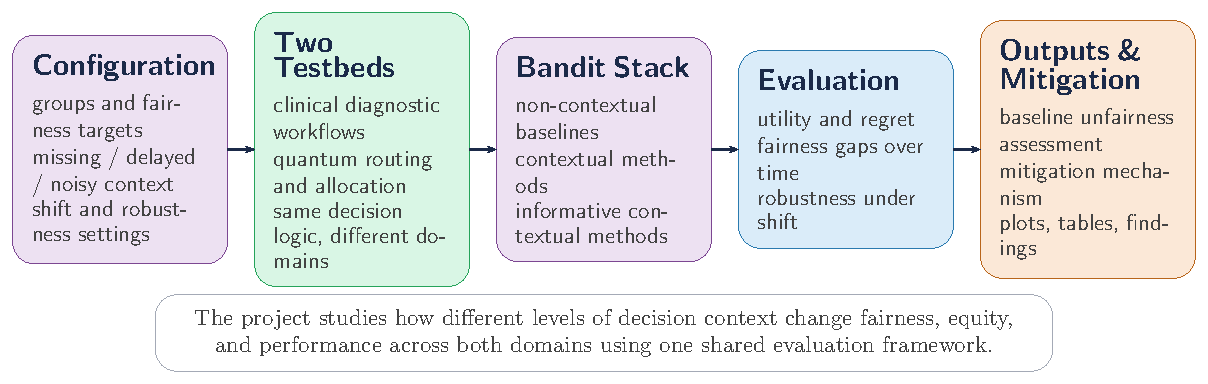
\includegraphics[width=0.97\linewidth]{proposal_framework_figure.pdf}
  \vspace{0.35em}

  \begin{block}{Why this matters}
    Same evaluation logic across both domains: configure $\rightarrow$ testbeds $\rightarrow$ methods $\rightarrow$ metrics $\rightarrow$ mitigation and findings.
  \end{block}
\end{frame}

\begin{frame}{Approach for the Next Two Semesters}
  \small
  \textcolor{TealAccent}{This is the implementation path for DSCI 601 and DSCI 602.}
  \vspace{0.5em}
  \begin{columns}[T,onlytextwidth]
    \column{0.49\textwidth}
      \begin{block}{DSCI 601: foundation}
        \begin{itemize}
          \item Build the clinical decision environment.
          \item Implement non-contextual and contextual baselines.
          \item Define utility and time-evolving fairness metrics.
          \item Add an initial mitigation mechanism and baseline-unfairness analysis.
        \end{itemize}
      \end{block}
    \column{0.49\textwidth}
      \begin{block}{DSCI 602: robustness and transfer}
        \begin{itemize}
          \item Integrate the quantum routing environment.
          \item Extend to informative contextual methods.
          \item Test robustness under distribution shift and adversarial conditions.
          \item Package code, evaluate transfer, and finalize the report/demo.
        \end{itemize}
      \end{block}
  \end{columns}
  \vspace{0.2em}
  \centering
  \scriptsize \textcolor{SoftGray}{Tools and workflow: Python, pandas/scikit-learn-style workflows, reproducible experiments, Colab/local/GCP, and simulation-first evaluation.}
\end{frame}

\begin{frame}{Expected Contribution}
  \small
  \textcolor{TealAccent}{The goal is not just a model, but a reusable fairness-aware decision framework.}
  \vspace{0.5em}
  \begin{itemize}
    \item A shared evaluation framework for fairness-aware sequential decision-making across two structurally similar but technically different domains.
    \item Evidence for when better context improves fairness and when explicit mitigation is still necessary.
    \item A clearer path from fairness-aware research toward reproducible implementation in future dissertation work.
  \end{itemize}
  \vspace{0.5em}
  \begin{block}{Takeaway}
    Fairness should be part of how sequential decision systems are designed and evaluated, not something added only after optimization is complete.
  \end{block}
  \vspace{0.2em}
  \centering
  \textcolor{DeepNavy}{Questions? \textbullet\ pizg8794@g.rit.edu}
\end{frame}

\end{document}
